\documentclass[11pt]{article}
\usepackage[margin=1in]{geometry}
\usepackage{amsmath,amssymb}
\usepackage{lmodern}
\usepackage[T1]{fontenc}
\usepackage{enumitem}
\usepackage{microtype}
\usepackage{tikz}
\usetikzlibrary{arrows.meta,angles,quotes,calc,decorations.pathreplacing}

\title{2018A F=ma Exam Review}
\author{Nathan P.}
\date{January 30, 2026}

\begin{document}
\maketitle

\section*{Problem 4}
To maximize the total $E$, you want to add the max KE, so the most effective place is perigee (same impulse, same $\Delta v$) because $\Delta K\propto v^2$, and $\Delta K$ would be larger if $v$ was already large:
\[
(100+5)^2-100^2>(10+5)^2-10^2
\]
(an example where $\Delta v=5$).

\section*{Problem 5}
Consider the fact that there are no net external horizontal forces, so the com doesn't move horizontally.

\section*{Problem 8}
Considering the IAOR to be the contact point, the top of the disk is always at $2v_{cm}$, because $v_{cm}-r\omega=0$ for it to roll without slipping, so $v_{cm}=r\omega$, and the top of the disk is at $2v_{cm}$.

\begin{center}
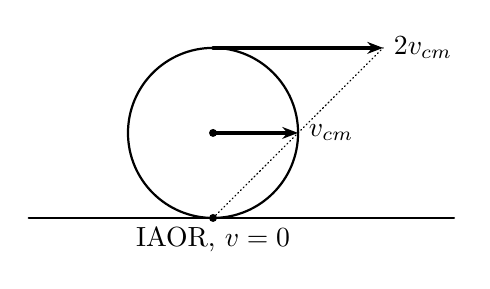
\begin{tikzpicture}[scale=0.9, line cap=round, line join=round, >={Stealth[length=2mm]}]
  \draw[thick] (-2.6,0) -- (3.4,0);
  \draw[thick] (0,1.2) circle (1.2);
  \fill (0,1.2) circle (1.6pt);
  \fill (0,0) circle (1.6pt) node[below] {IAOR, $v=0$};
  \draw[->, very thick] (0,1.2) -- (1.2,1.2) node[right] {$v_{cm}$};
  \draw[->, very thick] (0,2.4) -- (2.4,2.4) node[right] {$2v_{cm}$};
  \draw[densely dotted] (0,0) -- (2.4,2.4);
\end{tikzpicture}
\end{center}

\section*{Problem 10}
Think about the full picture. Identify what the graph should look like at the beginning, middle, and end, not just at one or two parts.

\section*{Problem 14}
\[
\frac{T_1}{T_2}=\frac{\omega_2}{\omega_1}=\frac{\sqrt{I_1}}{\sqrt{I_2}}=\frac{\sqrt{3m\ell^2}}{\sqrt{m\ell^2}}=\sqrt3.
\]
$mgd$ is the same for both ($3mg(L/3)$). ($d=L/3$ if you find $x_{cm}$, but it's actually unnecessary because $mgd$ is the same for both and would cancel out. In these ratio problems you can often think in terms of proportionality.)

\section*{Problem 24}
It initially increases because a larger-angle pendulum takes longer (by a factor of $1+\theta^2/16+\cdots$), but if you keep giving the mass a larger $K$, it'll swing in a circle, so of course the period of the motion would start decreasing once the circle gets completed at faster speeds.

\section*{Problem 25}
\begin{itemize}[leftmargin=*, itemsep=0.25em]
\item 1: $0.008/1.013=0.79\%$
\item 2: $\sqrt{(0.008/1.013)^2+(0.016/0.997)^2}\,/\,2=0.89\%$
\item 3: $\sqrt{\big(4(0.008/1.013)\big)^2+(0.016/0.997)^2}\,/\,5=0.71\%$
\end{itemize}
So $3<1<2$. Faster: Bob's period uncertainty is twice Alice's $\Delta t$, so Bob has $2\Delta t$ uncertainty, and you don't even need to plug in numbers:
\begin{itemize}[leftmargin=*, itemsep=0.25em]
\item 1: $\Delta t$
\item 2: $\sqrt{(\Delta t)^2+(2\Delta t)^2}\,/\,2=\frac{\sqrt5}{2}\Delta t=1.1\,\Delta t$
\item 3: $\sqrt{(4\Delta t)^2+(2\Delta t)^2}\,/\,5=\frac{2\sqrt5}{5}\Delta t=0.9\,\Delta t$
\end{itemize}

\end{document}
